%%%%%%%%%%%%%%%%%%%%%%%%%%%%%%%%%%%%%%%%%%%%%%%%%%%%%%%%%%%%%%%%%%%%%%%%%%%%%%%%%%
\begin{frame}[fragile]\frametitle{}
\begin{center}
{\Large Data Preprocessing with Scikit-Learn}
\end{center}
\end{frame}

%%%%%%%%%%%%%%%%%%%%%%%%%%%%%%%%%%%%%%%%%%%%%%%%%%%%%%%%%%%%%%%%%%%%%%%%%%%%%%%%%%
\begin{frame}[fragile]\frametitle{}
\begin{center}
{\Large Data Preprocessing for Pima-Indians Diabetis Dataset}

{\tiny (Ref: How To Prepare Your Data For Machine Learning in Python with Scikit-Learn - Jason Brownlee)}
\end{center}
\end{frame}

%%%%%%%%%%%%%%%%%%%%%%%%%%%%%%%%%%%%%%%%%%%%%%%%%%%%%%%%%%%
\begin{frame}[fragile]\frametitle{Read Data}
Import Pima Inidans dataset and split into Features (X) and target (Y)
\begin{lstlisting}
import pandas
import scipy
import numpy

url = "https://raw.githubusercontent.com/jbrownlee/Datasets/master/ pima-indians-diabetes.data.csv"
names = ['preg', 'plas', 'pres', 'skin', 'test', 'mass', 'pedi', 'age', 'class']

dataframe = pandas.read_csv(url, names=names)
array = dataframe.values

# separate array into input and output components
X = array[:,0:8]
Y = array[:,8]
\end{lstlisting}
\end{frame}

%%%%%%%%%%%%%%%%%%%%%%%%%%%%%%%%%%%%%%%%%%%%%%%%%%%%%%%%%%%
\begin{frame}[fragile]\frametitle{Rescale Data}

	\begin{itemize}
	\item Referred to as normalization and attributes are often rescaled into the range between 0 and 1. 
	\item This is useful for optimization algorithms in used in the core of machine learning algorithms like gradient descent. 
	\item It is also useful for algorithms that weight inputs like regression and neural networks and algorithms that use distance measures like K-Nearest Neighbors.
	\end{itemize}
	
\end{frame}

%%%%%%%%%%%%%%%%%%%%%%%%%%%%%%%%%%%%%%%%%%%%%%%%%%%%%%%%%%%
\begin{frame}[fragile]\frametitle{Rescale Data}
Rescale your data using scikit-learn using the MinMaxScaler class.
\begin{lstlisting}
# Rescale data (between 0 and 1)
from sklearn.preprocessing import MinMaxScaler

scaler = MinMaxScaler(feature_range=(0, 1))
rescaledX = scaler.fit_transform(X)

# summarize transformed data
numpy.set_printoptions(precision=3)
print(rescaledX[0:5,:])
\end{lstlisting}
\end{frame}

%%%%%%%%%%%%%%%%%%%%%%%%%%%%%%%%%%%%%%%%%%%%%%%%%%%%%%%%%%%
\begin{frame}[fragile]\frametitle{Rescale Data}
After rescaling you can see that all of the values are in the range between 0 and 1.
\begin{lstlisting}
[[ 0.353  0.744  0.59   0.354  0.     0.501  0.234  0.483]
 [ 0.059  0.427  0.541  0.293  0.     0.396  0.117  0.167]
 [ 0.471  0.92   0.525  0.     0.     0.347  0.254  0.183]
 [ 0.059  0.447  0.541  0.232  0.111  0.419  0.038  0.   ]
 [ 0.     0.688  0.328  0.354  0.199  0.642  0.944  0.2  ]]
\end{lstlisting}
\end{frame}


%%%%%%%%%%%%%%%%%%%%%%%%%%%%%%%%%%%%%%%%%%%%%%%%%%%%%%%%%%%
\begin{frame}[fragile]\frametitle{Standardize Data}

	\begin{itemize}
	\item Standardization is a useful technique to transform attributes with a Gaussian distribution and differing means and standard deviations to a standard Gaussian distribution with a mean of 0 and a standard deviation of 1.
	\item It is most suitable for techniques that assume a Gaussian distribution in the input variables and work better with rescaled data, such as linear regression, logistic regression and linear discriminate analysis.
	\end{itemize}
	
\end{frame}

%%%%%%%%%%%%%%%%%%%%%%%%%%%%%%%%%%%%%%%%%%%%%%%%%%%%%%%%%%%
\begin{frame}[fragile]\frametitle{Standardize Data}
Standardize data using scikit-learn with the StandardScaler class.
\begin{lstlisting}
# Standardize data (0 mean, 1 stdev)
from sklearn.preprocessing import StandardScaler

scaler = StandardScaler().fit(X)
rescaledX = scaler.transform(X)

# summarize transformed data
numpy.set_printoptions(precision=3)
print(rescaledX[0:5,:])
\end{lstlisting}
\end{frame}

%%%%%%%%%%%%%%%%%%%%%%%%%%%%%%%%%%%%%%%%%%%%%%%%%%%%%%%%%%%
\begin{frame}[fragile]\frametitle{Standardize Data}
The values for each attribute now have a mean value of 0 and a standard deviation of 1.
\begin{lstlisting}
[[ 0.64   0.848  0.15   0.907 -0.693  0.204  0.468  1.426]
 [-0.845 -1.123 -0.161  0.531 -0.693 -0.684 -0.365 -0.191]
 [ 1.234  1.944 -0.264 -1.288 -0.693 -1.103  0.604 -0.106]
 [-0.845 -0.998 -0.161  0.155  0.123 -0.494 -0.921 -1.042]
 [-1.142  0.504 -1.505  0.907  0.766  1.41   5.485 -0.02 ]]
\end{lstlisting}
\end{frame}




%%%%%%%%%%%%%%%%%%%%%%%%%%%%%%%%%%%%%%%%%%%%%%%%%%%%%%%%%%%
\begin{frame}[fragile]\frametitle{Normalize Data}

	\begin{itemize}
	\item Normalizing in scikit-learn refers to rescaling each observation (row) to have a length of 1 (called a unit norm in linear algebra).
	\item This preprocessing can be useful for sparse datasets (lots of zeros) with attributes of varying scales when using algorithms that weight input values such as neural networks and algorithms that use distance measures such as K-Nearest Neighbors.
	\end{itemize}
	
\end{frame}

%%%%%%%%%%%%%%%%%%%%%%%%%%%%%%%%%%%%%%%%%%%%%%%%%%%%%%%%%%%
\begin{frame}[fragile]\frametitle{Normalize Data}
Normalize data in Python with scikit-learn using the Normalizer class.
 \begin{lstlisting}
# Normalize data (length of 1)
from sklearn.preprocessing import Normalizer

scaler = Normalizer().fit(X)
normalizedX = scaler.transform(X)
# summarize transformed data
numpy.set_printoptions(precision=3)
print(normalizedX[0:5,:])
\end{lstlisting}
\end{frame}

%%%%%%%%%%%%%%%%%%%%%%%%%%%%%%%%%%%%%%%%%%%%%%%%%%%%%%%%%%%
\begin{frame}[fragile]\frametitle{Normalize Data}
The rows are normalized to length 1.
\begin{lstlisting}
[[ 0.64   0.848  0.15   0.907 -0.693  0.204  0.468  1.426]
 [-0.845 -1.123 -0.161  0.531 -0.693 -0.684 -0.365 -0.191]
 [ 1.234  1.944 -0.264 -1.288 -0.693 -1.103  0.604 -0.106]
 [-0.845 -0.998 -0.161  0.155  0.123 -0.494 -0.921 -1.042]
 [-1.142  0.504 -1.505  0.907  0.766  1.41   5.485 -0.02 ]]
\end{lstlisting}
\end{frame}



%%%%%%%%%%%%%%%%%%%%%%%%%%%%%%%%%%%%%%%%%%%%%%%%%%%%%%%%%%%
\begin{frame}[fragile]\frametitle{Binarize Data (Make Binary)}

	\begin{itemize}
	\item You can transform your data using a binary threshold. All values above the threshold are marked 1 and all equal to or below are marked as 0.
	\item This is called binarizing your data or threshold your data. It can be useful when you have probabilities that you want to make crisp values. 
	\item It is also useful when feature engineering and you want to add new features that indicate something meaningful.
	\end{itemize}
	
\end{frame}

%%%%%%%%%%%%%%%%%%%%%%%%%%%%%%%%%%%%%%%%%%%%%%%%%%%%%%%%%%%
\begin{frame}[fragile]\frametitle{Normalize Data}
Create new binary attributes in Python using scikit-learn with the Binarizer class.
\begin{lstlisting}
# binarization
from sklearn.preprocessing import Binarizer

binarizer = Binarizer(threshold=0.0).fit(X)
binaryX = binarizer.transform(X)
# summarize transformed data
numpy.set_printoptions(precision=3)
print(binaryX[0:5,:])
\end{lstlisting}
\end{frame}

%%%%%%%%%%%%%%%%%%%%%%%%%%%%%%%%%%%%%%%%%%%%%%%%%%%%%%%%%%%
\begin{frame}[fragile]\frametitle{Normalize Data}
You can see that all values equal or less than 0 are marked 0 and all of those above 0 are marked 1.
\begin{lstlisting}
[[ 1.  1.  1.  1.  0.  1.  1.  1.]
 [ 1.  1.  1.  1.  0.  1.  1.  1.]
 [ 1.  1.  1.  0.  0.  1.  1.  1.]
 [ 1.  1.  1.  1.  1.  1.  1.  1.]
 [ 0.  1.  1.  1.  1.  1.  1.  1.]]
\end{lstlisting}
\end{frame}








% %%%%%%%%%%%%%%%%%%%%%%%%%%%%%%%%%%%%%%%%%%%%%%%%%%%%%%%%%%%
% \begin{frame}[fragile]\frametitle{Kaggle Competition}

	% \begin{itemize}
	% \item Competition: https://www.kaggle.com/uciml/breast-cancer-wisconsin-data
	% \item Dataset: https://archive.ics.uci.edu/ml/datasets/Breast+ Cancer+ Wisconsin+ (Diagnostic)
	% \end{itemize}

% \begin{center}
% 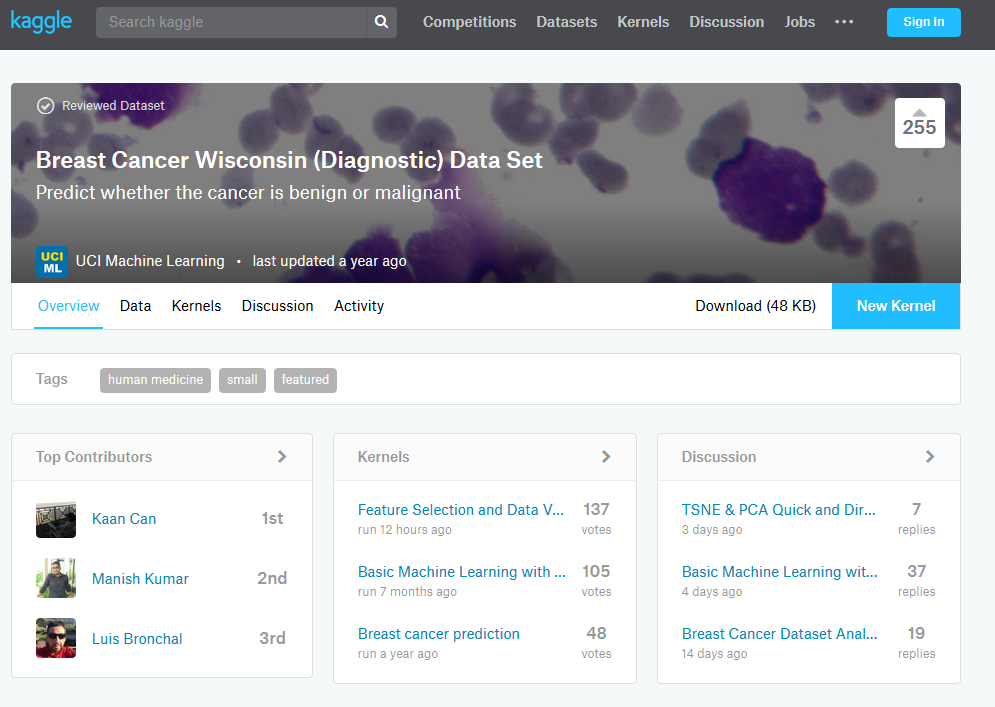
\includegraphics[width=0.45\linewidth,keepaspectratio]{kagglebc}
% \end{center}

% % Goal: Given parameters of cancer cells, predict malignant/benign
% \end{frame}

% %%%%%%%%%%%%%%%%%%%%%%%%%%%%%%%%%%%%%%%%%%%%%%%%%%%%%%%%%%%
% \begin{frame}[fragile]\frametitle{Identify the problem}
	% \begin{itemize}
	% \item Breast cancer is the most common malignancy among women, accounting for nearly 1 in 3 cancers diagnosed among women in the United States, and it is the second leading cause of cancer death among women. 
	% \item Breast Cancer occurs as a results of abnormal growth of cells in the breast tissue, commonly referred to as a Tumor. 
	% \item A tumor does not mean cancer - tumors can be benign (not cancerous), pre-malignant (pre-cancerous), or malignant (cancerous). 
	% \item Tests such as MRI, mammogram, ultrasound and biopsy are commonly used to diagnose breast cancer performed.
	% \end{itemize}
	
% {\tiny (Ref: Using Predictive Analysis To Predict Diagnosis of a Breast Tumor - Jean Njoroge)}
% \end{frame}

% %%%%%%%%%%%%%%%%%%%%%%%%%%%%%%%%%%%%%%%%%%%%%%%%%%%%%%%%%%%
% \begin{frame}[fragile]\frametitle{Expected outcome}
	% \begin{itemize}
	% \item Given breast cancer results from breast fine needle aspiration (FNA) test (is a quick and simple procedure to perform, which removes some fluid or cells from a breast lesion or cyst (a lump, sore or swelling) with a fine needle similar to a blood sample needle). 
	% \item Since this build a model that can classify a breast cancer tumor using two training classification:

	% \item 1= Malignant (Cancerous) - Present
	% \item 0= Benign (Not Cancerous) -Absent
	% \end{itemize}
	
% {\tiny (Ref: Using Predictive Analysis To Predict Diagnosis of a Breast Tumor - Jean Njoroge)}
% \end{frame}

% %%%%%%%%%%%%%%%%%%%%%%%%%%%%%%%%%%%%%%%%%%%%%%%%%%%%%%%%%%%
% \begin{frame}[fragile]\frametitle{Objective}
	% \begin{itemize}
	% \item Since the labels in the data are discrete, the predication falls into two categories, (i.e. Malignant or benign). 
	% \item In machine learning this is a classification problem.
	% \item {\it Thus, the goal is to classify whether the breast cancer is benign or malignant and predict the recurrence and non-recurrence of malignant cases after a certain period. To achieve this we have used machine learning classification methods to fit a function that can predict the discrete class of new input.}
	% \end{itemize}
	
% {\tiny (Ref: Using Predictive Analysis To Predict Diagnosis of a Breast Tumor - Jean Njoroge)}
% \end{frame}

% %%%%%%%%%%%%%%%%%%%%%%%%%%%%%%%%%%%%%%%%%%%%%%%%%%%%%%%%%%%
% \begin{frame}[fragile]\frametitle{Case Study: Cancer Dataset}
% \begin{center}
% 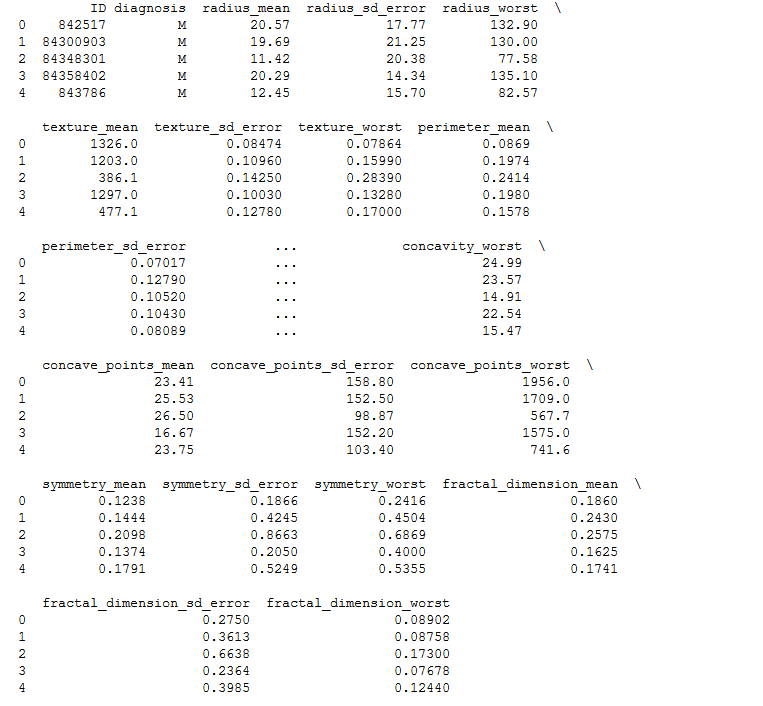
\includegraphics[width=\linewidth,keepaspectratio]{wbcd}
% \end{center}

% \end{frame}



% % %%%%%%%%%%%%%%%%%%%%%%%%%%%%%%%%%%%%%%%%%%%%%%%%%%%%%%%%%%%
% % \begin{frame}[fragile]\frametitle{Features}
% % \begin{center}
% % 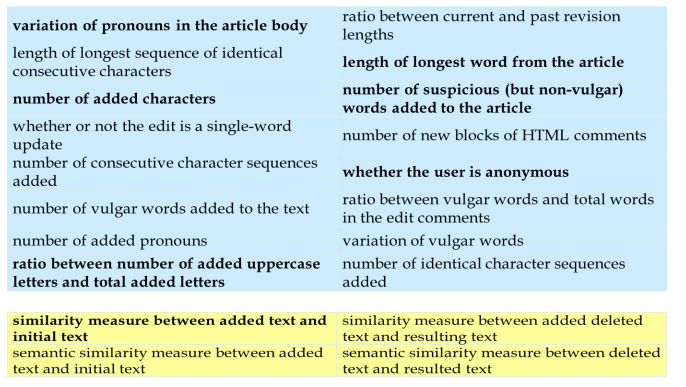
\includegraphics[width=0.8\linewidth,keepaspectratio]{features}
% % \end{center}
% % Are these ALL useful in predicting the tumor type?
% % \end{frame}

% %%%%%%%%%%%%%%%%%%%%%%%%%%%%%%%%%%%%%%%%%%%%%%%%%%%%%%%%%%%
% \begin{frame}[fragile]\frametitle{Redundancy}
	% \begin{itemize}
	% \item Some of the features could be dependent, so redundant
	% \item Needs dimension reduction to reduce feature space
	% \item {\bf While retaining most of the variance of the original data}
	% \end{itemize}
% \end{frame}

% %%%%%%%%%%%%%%%%%%%%%%%%%%%%%%%%%%%%%%%%%%%%%%%%%%%%%%%%%%%
% \begin{frame}[fragile]\frametitle{Case Study: Cancer Dataset}
% Import necessary libraries and load in the data file and header file provided
% \begin{lstlisting}
% import numpy  as np
% import csv
% import pandas as pd

% with open("data/field_names.txt","r") as header_data:
    % header_labels = [label.replace("\n",'') for label in header_data]
    
% print(header_labels)
% ['ID', 'diagnosis', 'radius_mean', 'radius_sd_error', ...,  'fractal_dimension_worst']
% \end{lstlisting}
% \end{frame}

% %%%%%%%%%%%%%%%%%%%%%%%%%%%%%%%%%%%%%%%%%%%%%%%%%%%%%%%%%%%
% \begin{frame}[fragile]\frametitle{Inspecting the data}
% The first step is to visually inspect the new data set. There are multiple ways to achieve this:


	% \begin{itemize}
	% \item The easiest being to request the first few records using the DataFrame data.head()* method. By default, “data.head()” returns the first 5 rows from the DataFrame object df (excluding the header row).
	% \item Alternatively, one can also use “df.tail()” to return the five rows of the data frame.
	% \item For both head and tail methods, there is an option to specify the number of records by including the required number in between the parentheses when calling either method.Inspecting the data
	% \end{itemize}
% \end{frame}

% %%%%%%%%%%%%%%%%%%%%%%%%%%%%%%%%%%%%%%%%%%%%%%%%%%%%%%%%%%%
% \begin{frame}[fragile]\frametitle{Case Study: Cancer Dataset}
% \begin{lstlisting}
% df = pd.read_csv("data/breast-cancer.csv")
% df.columns = header_labels
% print(df.head())

   % ID diagnosis  radius_mean  radius_sd_error  radius_worst  \
% 0    842517         M        20.57            17.77        132.90   
% 1  84300903         M        19.69            21.25        130.00   
% 2  84348301         M        11.42            20.38         77.58   
% 3  84358402         M        20.29            14.34        135.10   
% 4    843786         M        12.45            15.70         82.57   
% :
% \end{lstlisting}
% \end{frame}

% %%%%%%%%%%%%%%%%%%%%%%%%%%%%%%%%%%%%%%%%%%%%%%%%%%%%%%%%%%%
% \begin{frame}[fragile]\frametitle{Case Study: Cancer Dataset}
	% \begin{itemize}
	% \item The “info()” method provides a concise summary of the data; from the output, it provides the type of data in each column, the number of non-null values in each column, and how much memory the data frame is using.
	% \item The method get\_dtype_counts() will return the number of columns of each type in a DataFrame:
	% \end{itemize}


% \begin{lstlisting}
% df.info()
% <class 'pandas.core.frame.DataFrame'>
% RangeIndex: 569 entries, 0 to 568
% Data columns (total 32 columns):
% id                         569 non-null int64
% diagnosis                  569 non-null object          15.70         82.57   
% :
% \end{lstlisting}
% \end{frame}



% %%%%%%%%%%%%%%%%%%%%%%%%%%%%%%%%%%%%%%%%%%%%%%%%%%%%%%%%%%%
% \begin{frame}[fragile]\frametitle{Case Study: Cancer Dataset}

% \begin{lstlisting}
% print(df.shape)
% length = len(df)
% features = df.shape[1]-1
% malignant = len(df[df['diagnosis']=='M'])
% benign = len(df[df['diagnosis']=='B'])
% ratio = (float(malignant)/(length))*100

% print("{} rows".format(str(len(df))))
% print("{} features".format(features))
% print("{} diagnosed as malignant tumor".format(malignant))
% print("{} diagnosed as benign tumor".format(benign))
% print("{} percentage of malignant tumor".format(ratio))

% (568, 32)
% 568 rows
% 31 features
% 211 diagnosed as malignant tumor
% 357 diagnosed as benign tumor
% 37.147887323943664 percentage of malignant tumor
% \end{lstlisting}
% \end{frame}

% %%%%%%%%%%%%%%%%%%%%%%%%%%%%%%%%%%%%%%%%%%%%%%%%%%%%%%%%%%%
% \begin{frame}[fragile]\frametitle{Dimensionality of the Dataset}
	% \begin{itemize}
	% \item 568 rows/observations and 32 columns. 
	% \item Out of these 32, 1 is target and 31 are features
	% \item Out of 31 features, one is ``ID'' (not useful) so really there are 30 features/dimensions
	% \item {\bf Each row is a point in 30 Dimension space}
	% \end{itemize}
% \end{frame}

% %%%%%%%%%%%%%%%%%%%%%%%%%%%%%%%%%%%%%%%%%%%%%%%%%%%%%%%%%%%
% \begin{frame}[fragile]\frametitle{Case Study: Cancer Dataset}
% Basic descriptive statistics
% \begin{lstlisting}
% print(df.describe())
% \end{lstlisting}
% \begin{center}
% 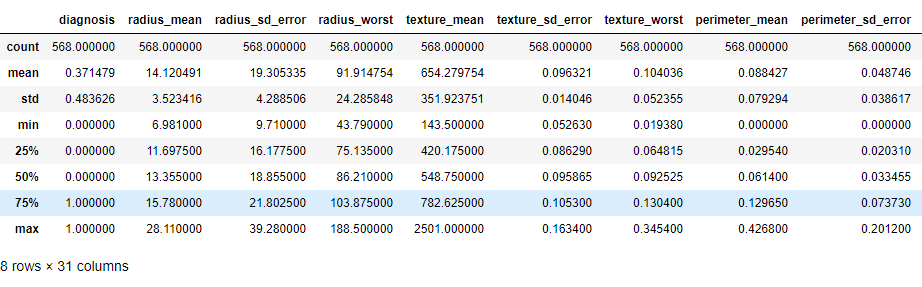
\includegraphics[width=0.8\linewidth,keepaspectratio]{data_prep1}
% \end{center}
% \end{frame}


% %%%%%%%%%%%%%%%%%%%%%%%%%%%%%%%%%%%%%%%%%%%%%%%%%%%%%%%%%%%
% \begin{frame}[fragile]\frametitle{Case Study: Cancer Dataset}
% Visualise distribution of data via histograms. Separate columns into smaller dataframes to perform visualization
% \begin{lstlisting}
% #Break up columns into groups, according to their suffix designation 
% #(_mean, _se,and __worst) to perform visualisation plots off. 
% #Join the 'ID' and 'Diagnosis' back on
% df_id_diag=df.loc[:,["id","diagnosis"]]
% df_diag=df.loc[:,["diagnosis"]]

% #For a merge + slice:
% df_mean=df.iloc[:,1:11]
% df_se=df.iloc[:,11:22]
% df_worst=df.iloc[:,23:]

% print(df_id_diag.columns)
% print(df_mean.columns)
% print(df_se.columns)
% print(df_worst.columns)
% \end{lstlisting}
% \end{frame}

% %%%%%%%%%%%%%%%%%%%%%%%%%%%%%%%%%%%%%%%%%%%%%%%%%%%%%%%%%%%
% \begin{frame}[fragile]\frametitle{Case Study: Cancer Dataset}
% \begin{lstlisting}
% Index(['id', 'diagnosis'], dtype='object')
% Index(['radius_mean', 'radius_sd_error', 'radius_worst', 'texture_mean',
       % 'texture_sd_error', 'texture_worst', 'perimeter_mean',
       % 'perimeter_sd_error', 'perimeter_worst', 'area_mean'],
      % dtype='object')
% Index(['area_sd_error', 'area_worst', 'smoothness_mean', 'smoothness_sd_error',
       % 'smoothness_worst', 'compactness_mean', 'compactness_sd_error',
       % 'compactness_worst', 'concavity_mean', 'concavity_sd_error',
       % 'concavity_worst'],
      % dtype='object')
% Index(['concave_points_sd_error', 'concave_points_worst', 'symmetry_mean',
       % 'symmetry_sd_error', 'symmetry_worst', 'fractal_dimension_mean',
       % 'fractal_dimension_sd_error', 'fractal_dimension_worst'],
      % dtype='object')
% \end{lstlisting}
% \end{frame}

% %%%%%%%%%%%%%%%%%%%%%%%%%%%%%%%%%%%%%%%%%%%%%%%%%%%%%%%%%%%
% \begin{frame}[fragile]\frametitle{Case Study: Cancer Dataset}
% Histogram the "_mean" suffix designition
% \begin{lstlisting}
% #Plot histograms of CUT1 variables
% hist_mean=df_mean.hist(bins=10, figsize=(15, 10),grid=False,)

% #Any individual histograms, use this:
% #df_cut['radius_worst'].hist(bins=100)
% \end{lstlisting}
% \end{frame}

% %%%%%%%%%%%%%%%%%%%%%%%%%%%%%%%%%%%%%%%%%%%%%%%%%%%%%%%%%%%
% \begin{frame}[fragile]\frametitle{Case Study: Cancer Dataset}
% Histogram the "_se" suffix designition
% \begin{lstlisting}
% #Plot histograms of _se variables
% hist_se=df_se.hist(bins=10, figsize=(15, 10),grid=False,)
% \end{lstlisting}
% \end{frame}

% %%%%%%%%%%%%%%%%%%%%%%%%%%%%%%%%%%%%%%%%%%%%%%%%%%%%%%%%%%%
% \begin{frame}[fragile]\frametitle{Case Study: Cancer Dataset}
% Histogram the "_worst" suffix designition
% \begin{lstlisting}
% #Plot histograms of _se variables
% hist_worst=df_worst.hist(bins=10, figsize=(15, 10),grid=False,)
% \end{lstlisting}
% \end{frame}

% %%%%%%%%%%%%%%%%%%%%%%%%%%%%%%%%%%%%%%%%%%%%%%%%%%%%%%%%%%%
% \begin{frame}[fragile]\frametitle{Observations}
	% \begin{itemize}
	% \item We can see that perhaps the attributes concavity,and concavity_point may have an exponential distribution ( ). 
	% \item We can also see that perhaps the texture and smooth and symmetry attributes may have a Gaussian or nearly Gaussian distribution. 
	% \item This is interesting because many machine learning techniques assume a Gaussian univariate distribution on the input variables.
	% \end{itemize}
% \end{frame}


% %%%%%%%%%%%%%%%%%%%%%%%%%%%%%%%%%%%%%%%%%%%%%%%%%%%%%%%%%%%
% \begin{frame}[fragile]\frametitle{Case Study: Cancer Dataset}
% Density Plot the "_mean" suffix designition
% \begin{lstlisting}
% plt = df_mean.plot(kind= 'density', subplots=True, layout=(4,3), sharex=False, 
                     % sharey=False,fontsize=12, figsize=(15,10))
% \end{lstlisting}
% \end{frame}

% %%%%%%%%%%%%%%%%%%%%%%%%%%%%%%%%%%%%%%%%%%%%%%%%%%%%%%%%%%%
% \begin{frame}[fragile]\frametitle{Case Study: Cancer Dataset}
% Density Plot the "_se" suffix designition
% \begin{lstlisting}
% plt = df_se.plot(kind= 'density', subplots=True, layout=(4,3), sharex=False, 
                     % sharey=False,fontsize=12, figsize=(15,10))
% \end{lstlisting}
% \end{frame}

% %%%%%%%%%%%%%%%%%%%%%%%%%%%%%%%%%%%%%%%%%%%%%%%%%%%%%%%%%%%
% \begin{frame}[fragile]\frametitle{Case Study: Cancer Dataset}
% Density Plot the "_worst" suffix designition
% \begin{lstlisting}
% plt = df_worst.plot(kind= 'density', subplots=True, layout=(4,3), sharex=False, 
                     % sharey=False,fontsize=12, figsize=(15,10))
% \end{lstlisting}
% \end{frame}
% %%%%%%%%%%%%%%%%%%%%%%%%%%%%%%%%%%%%%%%%%%%%%%%%%%%%%%%%%%%
% \begin{frame}[fragile]\frametitle{Observations}
	% \begin{itemize}
	% \item We can see that perhaps the attributes perimeter,radius, area, concavity,ompactness may have an exponential distribution ( ). 
	% \item We can also see that perhaps the texture and smooth and symmetry attributes may have a Gaussian or nearly Gaussian distribution. 
	% \item This is interesting because many machine learning techniques assume a Gaussian univariate distribution on the input variables.
	% \end{itemize}
% \end{frame}




% %%%%%%%%%%%%%%%%%%%%%%%%%%%%%%%%%%%%%%%%%%%%%%%%%%%%%%%%%%%
% \begin{frame}[fragile]\frametitle{Case Study: Cancer Dataset}
% Box Plot the "_mean" suffix designition
% \begin{lstlisting}
% plt = df_mean.plot(kind= 'box' , subplots=True, layout=(4,4), sharex=False, sharey=False,fontsize=12, figsize=(15,10))
% \end{lstlisting}
% \end{frame}

% %%%%%%%%%%%%%%%%%%%%%%%%%%%%%%%%%%%%%%%%%%%%%%%%%%%%%%%%%%%
% \begin{frame}[fragile]\frametitle{Case Study: Cancer Dataset}
% Box Plot the "_se" suffix designition
% \begin{lstlisting}
% plt = df_se.plot(kind= 'box' , subplots=True, layout=(4,4), sharex=False, sharey=False,fontsize=12, figsize=(15,10))
% \end{lstlisting}
% \end{frame}

% %%%%%%%%%%%%%%%%%%%%%%%%%%%%%%%%%%%%%%%%%%%%%%%%%%%%%%%%%%%
% \begin{frame}[fragile]\frametitle{Case Study: Cancer Dataset}
% Box Plot the "_worst" suffix designition
% \begin{lstlisting}
% plt = df_worst.plot(kind= 'box' , subplots=True, layout=(4,4), sharex=False, sharey=False,fontsize=12, figsize=(15,10))
% \end{lstlisting}
% \end{frame}
% %%%%%%%%%%%%%%%%%%%%%%%%%%%%%%%%%%%%%%%%%%%%%%%%%%%%%%%%%%%
% \begin{frame}[fragile]\frametitle{Observations}
	% \begin{itemize}
	% \item We can see that perhaps the attributes perimeter,radius, area, concavity,ompactness may have an exponential distribution ( ). 
	% \item We can also see that perhaps the texture and smooth and symmetry attributes may have a Gaussian or nearly Gaussian distribution. 
	% \item This is interesting because many machine learning techniques assume a Gaussian univariate distribution on the input variables.
	% \end{itemize}
% \end{frame}






























% %%%%%%%%%%%%%%%%%%%%%%%%%%%%%%%%%%%%%%%%%%%%%%%%%%%%%%%%%%%
% \begin{frame}[fragile]\frametitle{Case Study: Cancer Dataset}
% Need to have all columns except target, as real numeric. 
% \begin{lstlisting}
% df = df.set_index("ID")
% for col in df.columns:
    % if col != "diagnosis":
        % df[col] = pd.to_numeric(df[col])
% print(df.dtypes)
% print(df.radius_mean.mean())
% print(df.area_mean.mean())

% 14.1204911972
% 0.0627695950704
% \end{lstlisting}
% \end{frame}



% %%%%%%%%%%%%%%%%%%%%%%%%%%%%%%%%%%%%%%%%%%%%%%%%%%%%%%%%%%%
% \begin{frame}[fragile]\frametitle{Case Study: Cancer Dataset}
% Check for missing values
% \begin{lstlisting}
% print(pd.isnull(df).any())
% diagnosis                     False
% radius_mean                   False
% radius_sd_error               False
% radius_worst                  False
% texture_mean                  False
% texture_sd_error              False
% texture_worst                 False
% perimeter_mean                False
% perimeter_sd_error            False
% perimeter_worst               False
% area_mean                     False
% area_sd_error                 False
% ...
% symmetry_worst                False
% fractal_dimension_mean        False
% fractal_dimension_sd_error    False
% fractal_dimension_worst       False
% \end{lstlisting}
% \end{frame}

% %%%%%%%%%%%%%%%%%%%%%%%%%%%%%%%%%%%%%%%%%%%%%%%%%%%%%%%%%%%
% \begin{frame}[fragile]\frametitle{Case Study: Cancer Dataset}
% Leaving first (ie 0th) column, rest 31 are features. The first column is 'target'
% \begin{lstlisting}
% features = list(df.columns[2:32])
% print(features)
% target = df.columns[1:2]
% print(target)

% ['radius_mean', 'radius_sd_error', 'radius_worst', 'texture_mean', 'texture_sd_error', 'texture_worst', 'perimeter_mean', 'perimeter_sd_error', 'perimeter_worst', 'area_mean', 'area_sd_error', 'area_worst', 'smoothness_mean', 'smoothness_sd_error', 'smoothness_worst', 'compactness_mean', 'compactness_sd_error', 'compactness_worst', 'concavity_mean', 'concavity_sd_error', 'concavity_worst', 'concave_points_mean', 'concave_points_sd_error', 'concave_points_worst', 'symmetry_mean', 'symmetry_sd_error', 'symmetry_worst', 'fractal_dimension_mean', 'fractal_dimension_sd_error', 'fractal_dimension_worst']
% Index(['diagnosis'], dtype='object')
% \end{lstlisting}
% \end{frame}

% %%%%%%%%%%%%%%%%%%%%%%%%%%%%%%%%%%%%%%%%%%%%%%%%%%%%%%%%%%%
% \begin{frame}[fragile]\frametitle{Case Study: Cancer Dataset}
% There could be many features which are correlated
% \begin{lstlisting}
% import seaborn as sns
% import matplotlib.pyplot as plt

% f, ax = plt.subplots(figsize=(10, 8))
% corr = df.corr()
% sns.heatmap(corr, mask=np.zeros_like(corr, dtype=np.bool), cmap=sns.diverging_palette(220, 10, as_cmap=True),
            % square=True, ax=ax)
% plt.show()
% \end{lstlisting}
% \end{frame}

% %%%%%%%%%%%%%%%%%%%%%%%%%%%%%%%%%%%%%%%%%%%%%%%%%%%%%%%%%%%
% \begin{frame}[fragile]\frametitle{Feature Dependence by Correlation}
	% \begin{center}
% 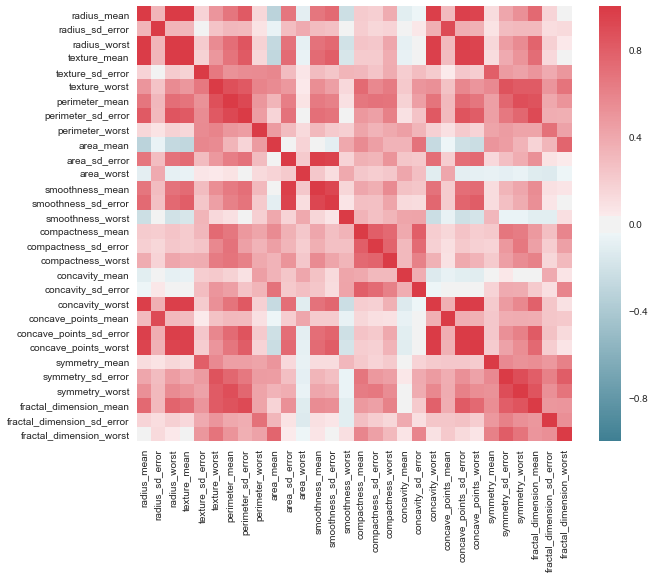
\includegraphics[width=0.8\linewidth,keepaspectratio]{correlation}
% \end{center}	
% \end{frame}

% %%%%%%%%%%%%%%%%%%%%%%%%%%%%%%%%%%%%%%%%%%%%%%%%%%%%%%%%%%%
% \begin{frame}[fragile]\frametitle{Case Study: Cancer Dataset}
% There could be many features which are correlated
% \begin{lstlisting}
% import matplotlib.pyplot as plt
% fig, ax = plt.subplots(1)
% for i in range(1):
    % x=df['radius_mean'],
    % y=df['concavity_worst'],
    % marker='o', 
    % alpha=0.3,
    % ax.scatter(x,y, label=str(i))
% plt.ylabel("radius_mean")
% plt.xlabel("concavity_worst")
% plt.legend(loc="best")
% plt.title("Any correlation?")
% plt.show()
% \end{lstlisting}
% \end{frame}

% %%%%%%%%%%%%%%%%%%%%%%%%%%%%%%%%%%%%%%%%%%%%%%%%%%%%%%%%%%%
% \begin{frame}[fragile]\frametitle{Any correlation?}
	% \begin{center}
% 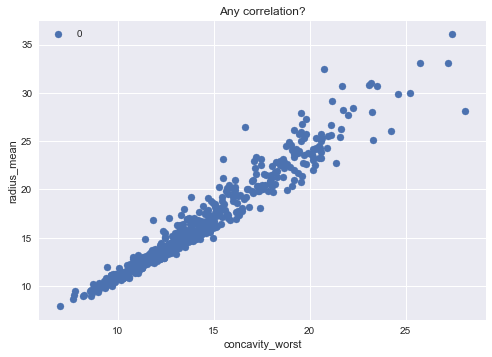
\includegraphics[width=0.7\linewidth,keepaspectratio]{corr1}
% \end{center}	
% Clear correlation between radius\_mean and concavity\_worst. One of them can be droppped from X, for training.
% \end{frame}

% %%%%%%%%%%%%%%%%%%%%%%%%%%%%%%%%%%%%%%%%%%%%%%%%%%%%%%%%%%%
% \begin{frame}[fragile]\frametitle{Case Study: Cancer Dataset}
% There could be many features which are correlated
% \begin{lstlisting}
% import matplotlib.pyplot as plt
% fig, ax = plt.subplots(1)
% for i in range(1):
    % x=df['area_mean']
    % y=df['concavity_worst'],
    % ax.scatter(x,y, label=str(i))
% plt.ylabel("area_mean")
% plt.xlabel("concavity_worst")
% plt.legend(loc="best")
% plt.title("Any correlation?")
% plt.show()
% \end{lstlisting}
% \end{frame}

% %%%%%%%%%%%%%%%%%%%%%%%%%%%%%%%%%%%%%%%%%%%%%%%%%%%%%%%%%%%
% \begin{frame}[fragile]\frametitle{Any correlation?}
	% \begin{center}
% 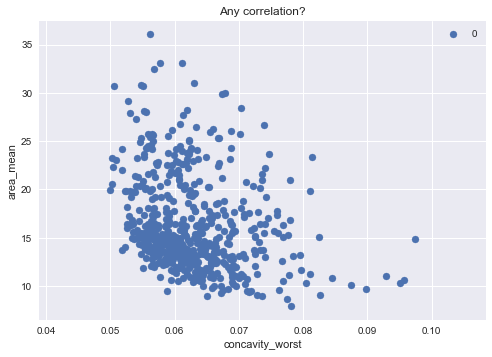
\includegraphics[width=0.7\linewidth,keepaspectratio]{corr2}
% \end{center}	
% There is no correlation between concavity\_worst and area\_mean and thus, both can be part of the features for training.
% \end{frame}

% %%%%%%%%%%%%%%%%%%%%%%%%%%%%%%%%%%%%%%%%%%%%%%%%%%%%%%%%%%%
% \begin{frame}[fragile]\frametitle{Case Study: Cancer Dataset}
% Create X and y for training and print their shapes just to make sure that we have all the data
% \begin{lstlisting}
% cleanup_nums = {'diagnosis':{"M": 1, "B": 0}}

% df.replace(cleanup_nums, inplace=True)
% Xdf = df[features]
% Ydf = df[target]

% print(Xdf.shape)
% print(Ydf.shape)

% (568, 30)
% (568, 1)
% \end{lstlisting}
% \end{frame}

% %%%%%%%%%%%%%%%%%%%%%%%%%%%%%%%%%%%%%%%%%%%%%%%%%%%%%%%%%%%
% \begin{frame}[fragile]\frametitle{Case Study: Cancer Dataset: Cross Validation}
% Lets start with cross-validation splits. This splits X itself into training and testing, so that we can measure accuracy like metrics.
% \begin{lstlisting}
% from sklearn.model_selection import train_test_split

% num_train = 450
% num_test = Xdf.shape[0] - num_train

% X_train, X_test, Y_train, Y_test = train_test_split(Xdf.values, Ydf.values, test_size=num_test, random_state=40)

% print("Training: {} rows.".format(X_train.shape[0]))
% print("Testing: {} rows.".format(X_test.shape[0]))
% print(X_train)
% print(Y_train)
% \end{lstlisting}
% \end{frame}

% % %%%%%%%%%%%%%%%%%%%%%%%%%%%%%%%%%%%%%%%%%%%%%%%%%%%%%%%%%%%
% % \begin{frame}[fragile]\frametitle{Case Study: Cancer Dataset: Modeling}
% % \begin{lstlisting}
% % from sklearn.metrics import fbeta_score, accuracy_score

% % def train_predict(learner, sample_size, X_train, y_train, X_test, y_test): 
    % % results = {}
    % % learner = learner.fit(X_train[:sample_size], y_train[:sample_size])
    % % predictions_test = learner.predict(X_test) # Predictions from test set
    % % predictions_train = learner.predict(X_train[:300]) # Predictions from the first 300 values in the training set
    % % results['acc_train'] = accuracy_score(y_train[:300], predictions_train)
    % % results['acc_test'] = accuracy_score(y_test, predictions_test)
    % % results['f_train'] = fbeta_score(y_train[:300], predictions_train, beta)
    % % results['f_test'] = fbeta_score(y_test, predictions_test, beta)
    % % print "{} trained on {} samples.".format(learner.__class__.__name__, sample_size)
    % % print "\tacc_train:{}\n\tacc_test:{}\n\tf_train:{}\n\tf_test:{}\n\tpred_time:{}".format(
        % % results['acc_train'], results['acc_test'], results['f_train'], results['f_test'], results['pred_time'])
    
    % % return results
% % \end{lstlisting}
% % \end{frame}


% % %%%%%%%%%%%%%%%%%%%%%%%%%%%%%%%%%%%%%%%%%%%%%%%%%%%%%%%%%%%
% % \begin{frame}[fragile]\frametitle{Case Study: Cancer Dataset: Modeling}
% % Lets start with cross-validation splits. This splits X itself into training and testing, so that we can measure accuracy like metrics.
% % \begin{lstlisting}
% % clf = DecisionTreeClassifier(min_samples_split=50)
% % train_predict(clf, X_train, Y_train, X_test, Y_test)

% % F1 training 0.9129.
% % F1 test 0.9362.
% % \end{lstlisting}
% % \end{frame}

% %%%%%%%%%%%%%%%%%%%%%%%%%%%%%%%%%%%%%%%%%%%%%%%%%%%%%%%%%%%
% \begin{frame}[fragile]\frametitle{Case Study: Cancer Dataset: Summary}
	% \begin{itemize}
	% \item From the given data it was seen that out of 30 odd features, the most important ones deciding if the tumor is malignant one or not are: 'fractal\_dimension\_mean', 'concavity\_worst','radius\_mean', 'concave\_points\_sd\_error', 'perimeter\_mean' and 'texture\_mean'.
	% \item So, form this study it is pretty clear that just focusing on a few features could result into more reliable and speedy predictions of malignant/benign tumors.
	% \end{itemize}
% \end{frame}